% Proto board generation version 1 description
% Author: Michael Mekonnen

\documentclass[12pt]{amsart}

% Packages
\usepackage[pdftex]{graphicx}

% Custom commands
% None

\title{Proto Board Generation: Version 1}

\begin{document}

\today
\maketitle

\section{Introduction}

TODO

\section{Steps}

TODO

\subsection{Terms}

\subsubsection{Circuit}

TODO

\begin{figure}
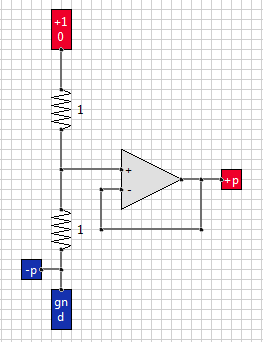
\includegraphics{Images/Circuit.png}
\caption{TODO}
\label{fig:circuit}
\end{figure}

\subsubsection{Circuit Piece}

TODO

\begin{figure}
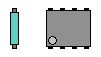
\includegraphics{Images/Circuit_Pieces.png}
\caption{TODO}
\label{fig:pieces}
\end{figure}

\subsubsection{Circuit Piece Placement}

TODO

\subsection{Circuit to Placement}

TODO

\begin{figure}
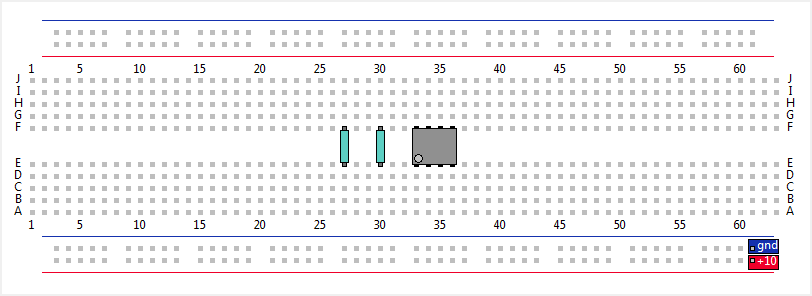
\includegraphics[width=\linewidth]{Images/Circuit_Piece_Placement.png}
\caption{TODO}
\label{fig:placement}
\end{figure}

\subsection{Placement to Wired Proto Board}

TODO

\begin{figure}
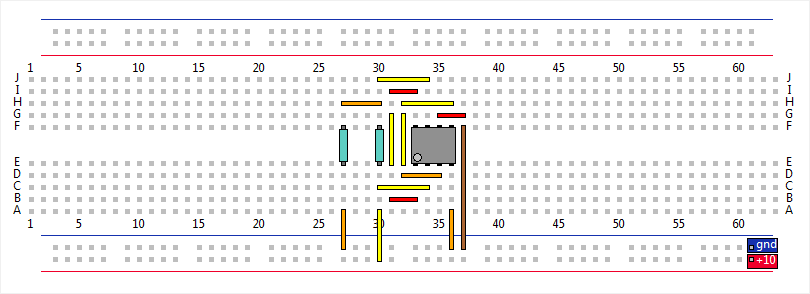
\includegraphics[width=\linewidth]{Images/Wired_Proto_Board.png}
\caption{TODO}
\label{fig:wired}
\end{figure}

\end{document}
